%%%%%%%%%%%%%%%%%%%%%%%%%%%%%%%%%%%%%%%%%%%%%%%%%%%%%%%%%%%%
% Name: XeTeX+xeCJK日常使用模板
% Author: Lox Freeman
% Email: xiaohanyu1988@gmail.com
%
% 本文档可以自由转载、修改,希望能给广大TeXer的中文之路提供一些方便。
%%%%%%%%%%%%%%%%%%%%%%%%%%%%%%%%%%%%%%%%%%%%%%%%%%%%%%%%%%%%

\documentclass[a4paper, 12pt]{article}

\usepackage{times}

% To add Chinese character encoding
\usepackage{xunicode, xltxtra}
\setmainfont[Mapping=tex-text]{AR PL KaitiM GB}
\setsansfont[Mapping=tex-text]{AR PL KaitiM GB}
\XeTeXlinebreaklocale "zh"

\makeatletter
\makeatother
\setlength{\parindent}{2em}%中文缩进两个汉字位
%中文断行
\XeTeXlinebreakskip = 0pt plus 1pt

%%%%%%%%%%%%%日常所用宏包、通通放在一起%%%%%%%%%%%%%%%%%%%%%%%%%%%%
% 什么常用的宏包都可以放这里。下面是我常用的宏包,每个都给出了简要注释
\usepackage[top=2.5cm, bottom=2cm, left=2cm, right=2cm]{geometry} % 控制页边距
\usepackage{enumerate}               % 控制项目列表
\usepackage{multicol}                % 多栏显示

\usepackage[%
    pdfstartview=FitH,%
    bookmarks=true,%
    bookmarksnumbered=true,%
    bookmarksopen=true,%
    colorlinks=true,%
    citecolor=blue,%
    linkcolor=blue,%
    anchorcolor=green,%
    urlcolor=blue%
]{hyperref}

\usepackage{titlesec}                % 控制标题
\usepackage{titletoc}                % 控制目录
\usepackage{type1cm}                 % 控制字体大小
\usepackage{indentfirst}             % 首行缩进,用\noindent取消某段缩进
\usepackage{cite}                    % 支持引用
\usepackage{color,xcolor}            % 支持彩色文本、底色、文本框等
\usepackage{latexsym}                % LaTeX一些特殊符号宏包
\usepackage{amsmath}                 % AMS LaTeX宏包
\usepackage{bm}                      % 数学公式中的黑斜体
\usepackage{relsize}                 % 调整公式字体大小:\mathsmaller, \mathlarger
%\makeindex                          % 生成索引

%%%%%%%%%%%%%%%%%%%%%%%%%基本插图方法%%%%%%%%%%%%%%%%%%%%%%%%%%%
\usepackage{graphicx}                % 图形宏包
% \begin{figure}[htbp]               % 控制插图位置
%   \setlength{\abovecaptionskip}{0pt}    
%   \setlength{\belowcaptionskip}{10pt}
                                     % 控制图形和上下文的距离
%   \centering                       % 使图形居中显示
%   \includegraphics[width=0.8\textwidth]{CTeXLive2008.jpg}
                                     % 控制图形显示宽度为0.8\textwidth
%   \caption{CTeXLive2008安装过程} \label{fig:CTeXLive2008}
                                     % 图形题目和交叉引用标签
% \end{figure}
%%%%%%%%%%%%%%%%%%%%%%%%%插图方法结束%%%%%%%%%%%%%%%%%%%%%%%%%%%


%%%%%%%%%%%%%%%%%%%%%%%%%fancyhdr设置页眉页脚%%%%%%%%%%%%%%%%%%%%
\usepackage{fancyhdr}                % 页眉页脚
\pagestyle{fancy}                    % 页眉页脚风格
\setlength{\headheight}{15pt}        % 有时会出现\headheight too small的warning
\fancyhf{}                          % 清空当前页眉页脚的默认设置
%%%%%%%%%%%%%%%%%%%%%%%%%fancyhdr设置结束%%%%%%%%%%%%%%%%%%%%%%%


%%%%%%%%%%%%%%%%%%%%%%%%%listings宏包粘贴源码%%%%%%%%%%%%%%%%%%%%
\usepackage{listings}                % 方便粘贴源代码,部分代码高亮功能
\lstloadlanguages{}                  % 所要粘贴代码的编程语言

%%%%设置listings宏包的一些全局样式%%%%
%%%%参见http://hi.baidu.com/shawpinlee/blog/item/9ec431cbae28e41cbe09e6e4.html%%%%
\lstset{
%numbers=left,
%numberstyle=\tiny,
basicstyle=\small\ttfamily,
keywordstyle=\color{blue!70}, commentstyle=\color{red!50!green!50!blue!50},
                                     % 关键字高亮
frame=shadowbox,                     % 给代码加框
rulesepcolor=\color{red!20!green!20!blue!20},
escapechar=`,                        % 中文逃逸字符
xleftmargin=2em,xrightmargin=2em, aboveskip=1em,
breaklines,                          % 这条命令可以让LaTeX自动将长的代码行换行排版
extendedchars=false                  % 这一条命令可以解决代码跨页时,章节标题,页眉等汉字不显示的问题
}
%%%%%%%%%%%%%%%%%%%%%%%%%listings宏包设置结束%%%%%%%%%%%%%%%%%%%%


%%%%%%%%%%%%%%%%%%%%%%%%%一些关于中文文档的重定义%%%%%%%%%%%%%%%%%

%%%%数学公式定理的重定义%%%%
\newtheorem{example}{例}                                   % 整体编号
\newtheorem{algorithm}{算法}
\newtheorem{theorem}{定理}[section]                         % 按 section 编号
\newtheorem{definition}{定义}
\newtheorem{axiom}{公理}
\newtheorem{property}{性质}
\newtheorem{proposition}{命题}
\newtheorem{lemma}{引理}
\newtheorem{corollary}{推论}
\newtheorem{remark}{注解}
\newtheorem{condition}{条件}
\newtheorem{conclusion}{结论}
\newtheorem{assumption}{假设}

%%%%章节等名称重定义%%%%
\renewcommand{\contentsname}{目录}     
\renewcommand{\indexname}{索引}
\renewcommand{\listfigurename}{插图目录}
\renewcommand{\listtablename}{表格目录}
\renewcommand{\figurename}{图}
\renewcommand{\tablename}{表}
\renewcommand{\appendixname}{附录}

%%%%设置chapter、section与subsection的格式%%%%
\titleformat{\chapter}{\centering\huge}{第\thechapter{}章}{1em}{\textbf}
%\titleformat{\section}{\centering\large}{\thesection}{1em}{\textbf}
\titleformat{\section}{\raggedright\large}{\thesection}{1em}{\textbf}
\titleformat{\subsection}{\huge}{\thesubsection}{1em}{\textbf}
%%%%%%%%%%%%%%%%%%%%%%%%%中文重定义结束%%%%%%%%%%%%%%%%%%%%


%%%%%%%%%%%%%%%%%%%%%%%%%一些个性设置%%%%%%%%%%%%%%%%%%%%%%
% \renewcommand{\baselinestretch}{1.3}     % 效果同\linespread{1.3}
% \pagenumbering{arabic}                   % 设定页码方式,包括arabic、roman等方式
% \sloppy                                  % 有时LaTeX无从断行,产生overfull的错误,
                                           % 这条命令降低LaTeX断行标准
\setlength{\parskip}{0.5\baselineskip}     % 设定段间距
\linespread{1.2}                           % 设定行距
\newcommand{\pozhehao}{\kern0.3ex\rule[0.8ex]{2em}{0.1ex}\kern0.3ex}
                                           % 中文破折号,据说来自清华模板

%%%%%%%%%%%%%%%%%%%%%%%%%个性设置结束%%%%%%%%%%%%%%%%%%%%%%


%%%%%%%%%%%%%%%%%%%%%%%%%正文部分%%%%%%%%%%%%%%%%%%%%%%%%%
\begin{document}
\setlength{\parindent}{2em}                    
% 设定首行缩进为2em。注意此设置一定要在document环境之中。
% 这可能与\setlength作用范围相关

\title{Windows XP下安装QT4开发环境}
\author{默之\\\textrm{yyhoo2.young@gmail.com}}
\date{2011年12月18日}
\maketitle

\section{下载QT SDK}
去QT官方网\footnote{\href{http://qt.nokia.com/downloads}{QT官方网下载页面}}下载最新版的QT SDK for Windows。

\section{安装QT}

QT SDK下载完毕后,点击qt-sdk-win-opensource-2010.02.1.exe文件,开始安装QT(根据向导提示安装,安装过程中进度有点慢,请耐心等待。。。)

\section{测试}
点击桌面上的QT Creator图标,启动QT Creator。

(1)点击菜单File->New File or Project,弹出一个New对话框,选择Projects下的Empty Qt4 Project选项,点击OK按钮,如下图所示:

\begin{center}
  \setlength{\abovecaptionskip}{0pt}    
  \setlength{\belowcaptionskip}{10pt}
  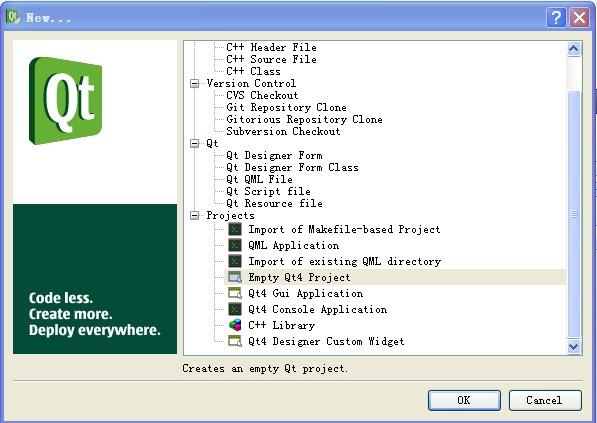
\includegraphics[width=0.5\textwidth]{qt01.jpg}
\end{center}


(2)创建 工程名hello,选择存放目录D:\textbackslash Qt\textbackslash 2010.02.1\textbackslash
qtprojects,然后点击Next按钮,如下图所示:

\begin{center}
  \setlength{\abovecaptionskip}{0pt}    
  \setlength{\belowcaptionskip}{10pt}
  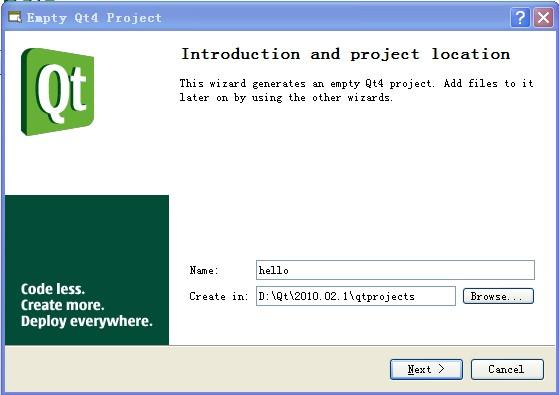
\includegraphics[width=0.5\textwidth]{qt02.jpg}
\end{center}

(3)点击 Finish按钮,成功创建一个空项目hello.pro

\begin{center}
  \setlength{\abovecaptionskip}{0pt}    
  \setlength{\belowcaptionskip}{10pt}
  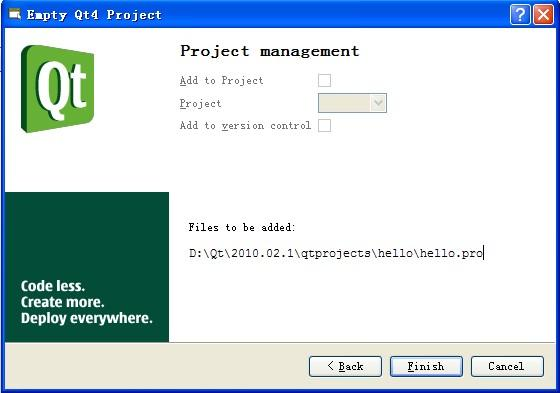
\includegraphics[width=0.5\textwidth]{qt03.jpg}
\end{center}

(4)点击菜单File->New File or Project,弹出一个New对话框,选 择 C++下的C++ Source File选项,点击OK按钮,如下图所示:

\begin{center}
  \setlength{\abovecaptionskip}{0pt}    
  \setlength{\belowcaptionskip}{10pt}
  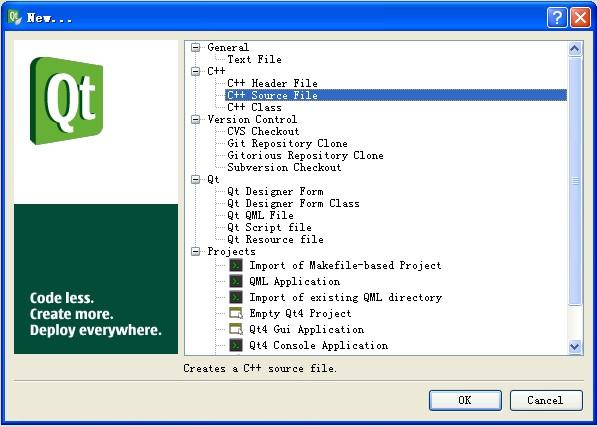
\includegraphics[width=0.5\textwidth]{qt04.jpg}
\end{center}

(5)创建 源文件hello.cpp,并选择存放目录(D:\textbackslash Qt\textbackslash 2010.02.1\textbackslash
qtprojects\textbackslash hello),然后点击Next按钮,如下图所示:

\begin{center}
  \setlength{\abovecaptionskip}{0pt}    
  \setlength{\belowcaptionskip}{10pt}
  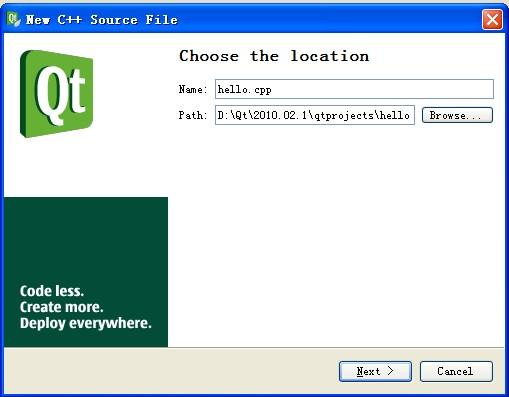
\includegraphics[width=0.5\textwidth]{qt05.jpg}
\end{center}

(6)工程管理,点击Finish按钮。

\begin{center}
  \setlength{\abovecaptionskip}{0pt}    
  \setlength{\belowcaptionskip}{10pt}
  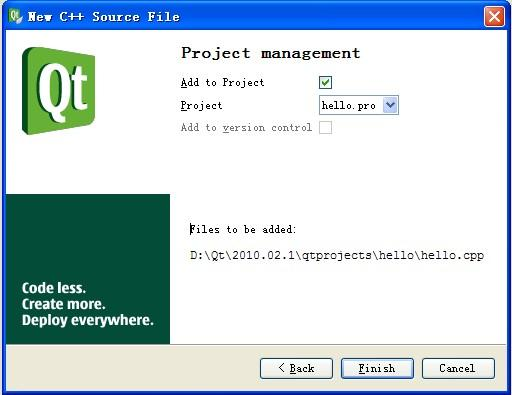
\includegraphics[width=0.5\textwidth]{qt06.jpg}
\end{center}

(7)点击 Projects视图中的hello.cpp,并编辑以下内容:

\begin{lstlisting}[language=C++]
#include <QApplication>
#include <QLabel>
 
int main(int argc, char *argv[]) {
    QApplication app(argc, argv);
 
    QLabel *label = new QLabel;
    label->setText("<center><h1>Hello World!</h1></center>");
    label->setWindowTitle("QT");
    label->resize(200, 50);
    label->show();
 
    return app.exec();
}
\end{lstlisting}

编辑完毕并保存。点击菜单Build->Build All或使用快捷键Ctrl+Shift+B编译工程;编译成功后,使用菜单Build->Run或快捷键Ctrl+R运行可执行文件 hello.exe,如下图所示:

\begin{center}
  \setlength{\abovecaptionskip}{0pt}    
  \setlength{\belowcaptionskip}{10pt}
  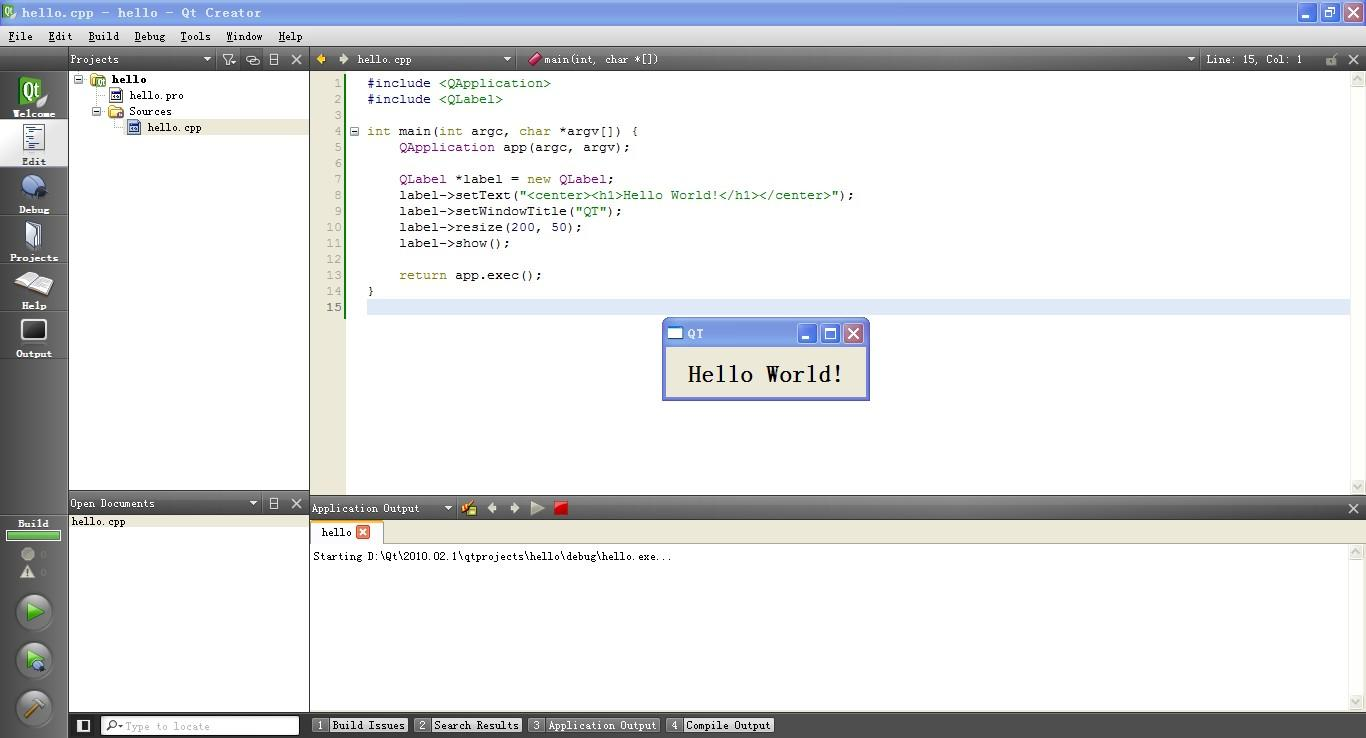
\includegraphics[width=0.5\textwidth]{qt07.jpg}
\end{center}

\begin{flushright}
默之 \\于2010年6月1日
\end{flushright}


\end{document}
%%%%%%%%%%%%%%%%%%%%%%%%%正文部分结束%%%%%%%%%%%%%%%%%%%%%%
